\documentclass[a4paper,12pt]{article}
\usepackage[T1]{fontenc}
\usepackage[utf8]{inputenc}
\usepackage{titlesec}
\usepackage{hyperref}
\usepackage{listings}
\usepackage{xcolor}
\usepackage{tocloft}
\usepackage{graphicx}
\usepackage{titling}
\usepackage{lmodern}
\usepackage{geometry}
\geometry{a4paper, margin=1in}

\newcommand{\sectionbreak}{\clearpage}

\hypersetup{
colorlinks=true,
linkcolor=blue,
urlcolor=red,
filecolor=green,
pdfborder={0 0 0},
citecolor=blue
}

\title{\textbf{Raspberry Pi 5 Projects} \\ \Large A Collection of Practical Applications}
\author{Tautminas Cibulskis}
\date{\today}

\begin{document}

\begin{titlepage}
\centering
\vspace*{2cm}
{\Huge \textbf{Raspberry Pi 5 Projects} \par}
\vspace{0.5cm}
{\Large A Collection of Practical Applications\par}
\vspace{2cm}
{\Large \textbf{Tautminas Cibulskis} \par}
\vspace{1.5cm}
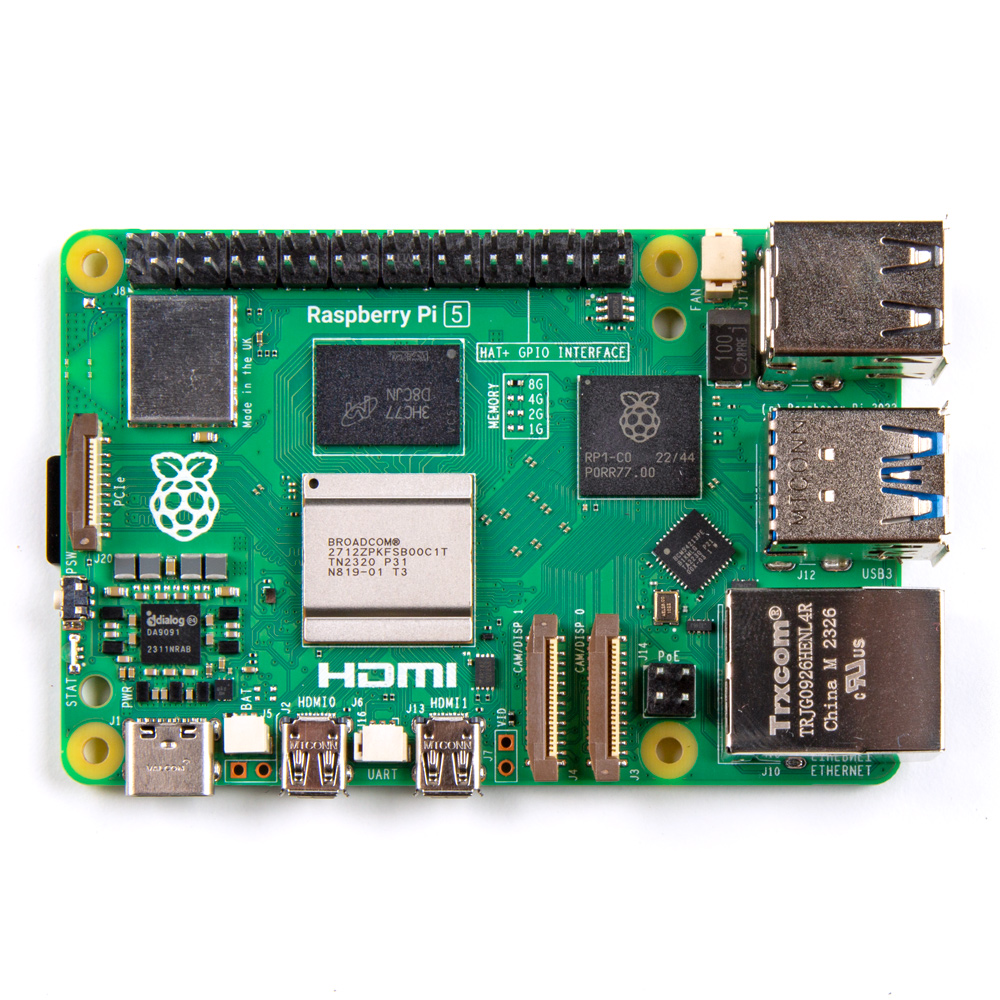
\includegraphics[width=0.6\textwidth]{images/raspberry-pi-5.jpg}
\vfill
{\large \today\par}
\end{titlepage}

\renewcommand{\cftsecleader}{\cftdotfill{\cftdotsep}}

\tableofcontents

\section*{\phantomsection About}
\addcontentsline{toc}{section}{About}

This document provides descriptions, instructions and commands for projects using a Raspberry Pi 5. Each project is inspired by a YouTube video, but this document refines and expands upon the content to offer clear guidance for those who wish to replicate the projects. The purpose of collecting this information in a single document is as follows:

\begin{itemize}
\item Some videos lack quality or are no longer relevant. This document selects the useful ones.
\item Some videos do not provide commands in written form. By providing them here, readers can avoid needing to manually retype everything.
\item Some videos could benefit from additional suggestions or improvements. This document expands on those projects to make them more practical.
\end{itemize}

The projects in this document were created using the Raspberry Pi 5 Desktop Kit. However, in most cases, a Raspberry Pi 5 Starter Kit provides all the necessary components to follow along. Additionally, these projects are not specific to the Raspberry Pi 5 as most of them can be completed using other Raspberry Pi models as well.  

Some instructions require specific values, for example, an IP address or cryptocurrency wallet address. These values are represented in the format \texttt{\textless EXAMPLE\_VALUE\textgreater}, with angle brackets and capitalization to indicate that they must be replaced with actual values. Blindly copying and pasting commands without replacing these placeholders will result in errors. Pay attention to the instructions and substitute the placeholders with the appropriate values.

In IT, a "project" is defined as a time-bound endeavour with a unique outcome. While this definition does not fully align with how it is used in the document, it remains the closest approximation to describe the work presented here.
\section*{\phantomsection Raspberry Pi 5 Preparation}
\addcontentsline{toc}{section}{Raspberry Pi 5 Preparation}

Before using your Raspberry Pi, you must first install an operating system onto a microSD card. Follow these steps to set it up:
\begin{enumerate}
\item Insert the microSD card into your PC (not the Raspberry Pi) using an SD adapter. Depending on the adapter, plug it into either the SD card slot or a USB port on your computer.
\item Open the \href{https://www.raspberrypi.com/software}{\textbf{\color{blue}Raspberry Pi Imager}} application. This tool simplifies the process of installing an operating system onto your Raspberry Pi’s storage. It has three main options:
\begin{itemize}
\item Device: Select your Raspberry Pi device (in this case, Raspberry Pi 5).
\item Operating System: Choose the OS based on the project’s requirements. The required OS is stated at the start of the project section.
\item Storage: Select the storage device (in this case, a microSD card) that will be used to boot the Raspberry Pi and store data. Be careful, as this process will erase all existing data on the selected storage device.
\end{itemize}
\item Customize the settings to enable remote access to the Raspberry Pi by pressing \texttt{Ctrl + Shift + X}. Then, set the hostname, username, password, configure the wireless LAN, set locale settings and enable SSH.
\item Proceed with the OS installation by selecting \textbf{Next}. The Raspberry Pi Imager will then write the OS to the selected storage device.
\item Once the OS is successfully written to the microSD card, insert it into the Raspberry Pi and power it on. Your Raspberry Pi will now be ready to use.
\end{enumerate}

For most projects, you'll need to connect to the Raspberry Pi remotely. To do so, follow these steps:
\begin{enumerate}
\item Use a tool like \href{https://www.fing.com/}{\textbf{\color{blue}Fing}}, available for both mobile and desktop, to find the Raspberry Pi's IP address. Fing detects devices on your local network and displays their IP addresses.
\item Once you have the IP address, connect to the Raspberry Pi via SSH. Use a tool like \href{https://www.chiark.greenend.org.uk/~sgtatham/putty/}{\textbf{\color{blue}PuTTY}}, a free SSH client for Windows. Launch PuTTY, enter the Raspberry Pi's IP address, select SSH as the connection type and click \textbf{Open}. Log in using your customized credentials (username and password) if you have set them, or use the default credentials (username: pi, password: raspberry) otherwise.
\end{enumerate}

After logging into your Raspberry Pi 5, either remotely or by directly accessing it, you need to run two essential commands that are recommended for every project:
\begin{enumerate}
\item \texttt{sudo apt update}: This command updates the list of available packages and their versions from the repositories.
\item \texttt{sudo apt upgrade}: This command upgrades all the installed packages to their latest available versions.
\end{enumerate}

You can run both commands at once by using:
\begin{verbatim} sudo apt update && sudo apt upgrade -y \end{verbatim}

The \texttt{-y} flag automatically confirms all prompts during the upgrade process, so you won't need to manually approve each step. This may take some time depending on your internet speed and the number of packages that need to be upgraded.
\section{Hosting a Dark Web Site}

\textbf{Video}: \href{https://www.youtube.com/watch?v=bllS9tkCkaM}{\textbf{\color{blue}i put a DARK WEB website on a Raspberry Pi!!}} (Channel: \href{https://www.youtube.com/@NetworkChuck}{\textbf{\color{blue}NetworkChuck}})

\vspace{0.5cm}

\noindent \textbf{Operating System}: Raspberry Pi OS Lite (64-bit), remote connection.

\vspace{0.5cm}

\noindent \textbf{Steps:}

\begin{enumerate}
\item Update package lists and install Tor:
\begin{lstlisting}[language=bash, breaklines=true, breakatwhitespace=true, columns=fullflexible]
$ sudo apt update
$ sudo apt install tor
\end{lstlisting}

\item Edit the Tor configuration file:
\begin{lstlisting}[language=bash, breaklines=true, breakatwhitespace=true, columns=fullflexible]
$ sudo nano /etc/tor/torrc
\end{lstlisting}
Uncomment the following lines:
\begin{lstlisting}[language=bash, breaklines=true, breakatwhitespace=true, columns=fullflexible]
HiddenServiceDir /var/lib/tor/hidden_service/
HiddenServicePort 80 127.0.0.1:80
\end{lstlisting}

\item Restart the Tor service:
\begin{lstlisting}[language=bash, breaklines=true, breakatwhitespace=true, columns=fullflexible]
$ sudo service tor stop
$ sudo service tor start
$ sudo service tor status
\end{lstlisting}

\item Obtain your site address:
\begin{lstlisting}[language=bash, breaklines=true, breakatwhitespace=true, columns=fullflexible]
$ sudo cat /var/lib/tor/hidden_service/hostname
\end{lstlisting}

\item Install and start Nginx:
\begin{lstlisting}[language=bash, breaklines=true, breakatwhitespace=true, columns=fullflexible]
$ sudo apt install nginx
$ sudo service nginx start
$ sudo service nginx status
\end{lstlisting}
You can now check your website using the .onion address from the previous step.

\item Modify Nginx configuration:
\begin{lstlisting}[language=bash, breaklines=true, breakatwhitespace=true, columns=fullflexible]
$ sudo nano /etc/nginx/nginx.conf
\end{lstlisting}
Uncomment the following lines:
\begin{lstlisting}[language=bash, breaklines=true, breakatwhitespace=true, columns=fullflexible]
port_in_redirect off;
server_name_in_redirect off;
\end{lstlisting}

Add the following line below "port\_in\_redirect off;":
\begin{lstlisting}[language=bash, breaklines=true, breakatwhitespace=true, columns=fullflexible]
server_tokens off;
\end{lstlisting}

\item Restart Nginx to apply changes:
\begin{lstlisting}[language=bash, breaklines=true, breakatwhitespace=true, columns=fullflexible]
$ sudo service nginx restart
\end{lstlisting}
Visit the site using your .onion address to check if the site works after the configuration changes.

\item Create a simple web page:
\begin{lstlisting}[language=bash, breaklines=true, breakatwhitespace=true, columns=fullflexible]
$ cd /var/www/html
$ sudo rm index.nginx-debian.html
$ sudo nano index.html
\end{lstlisting}
Add your HTML content and save the file.

\item Restart Nginx to apply changes:
\begin{lstlisting}[language=bash, breaklines=true, breakatwhitespace=true, columns=fullflexible]
$ sudo service nginx restart
\end{lstlisting}
Your site should now be accessible via your .onion address!
\end{enumerate}

\section{Mining Monero Cryptocurrency}

\noindent \textbf{Video}: \href{https://www.youtube.com/watch?v=hHtGN_JzoP8}{\textbf{\color{blue}How to Mine Monero on Raspberry Pi}} (Channel: \href{https://www.youtube.com/@NetworkChuck}{\textbf{\color{blue}NetworkChuck}})

\vspace{0.5cm}

\noindent \textbf{Operating System}: Raspberry Pi OS Lite (64-bit), remote connection.

\vspace{0.5cm}

\noindent \textbf{Steps:}
\begin{enumerate}
\item Update package lists and install dependencies:
\begin{lstlisting}[language=bash, breaklines=true, breakatwhitespace=true, columns=fullflexible]
$ sudo apt update
$ sudo apt install git build-essential cmake libuv1-dev libssl-dev libhwloc-dev -y
\end{lstlisting}

\item Clone the XMRig repository and build the miner:
\begin{lstlisting}[language=bash, breaklines=true, breakatwhitespace=true, columns=fullflexible]
$ git clone https://github.com/xmrig/xmrig.git
$ cd xmrig
$ mkdir build
$ cd build
$ cmake ..
$ make
\end{lstlisting}

\item Create a Monero (XMR) wallet: Download and install the Monero GUI Wallet from \href{https://www.getmonero.org}{\textbf{\color{blue}getmonero.org}}, choose Simple Mode, create a new wallet, name it, back up the mnemonic seed, set a password, and find your wallet address under the Account tab.

\item Start mining Monero:  
\begin{lstlisting}[language=bash, breaklines=true, breakatwhitespace=true, columns=fullflexible]
$ ./xmrig -o gulf.moneroocean.stream:10128 -u <YOUR_WALLET_ADDRESS> -p <WORKER_NAME>
\end{lstlisting}

Use the following keys to monitor mining in real time:  
\begin{itemize}
\item \texttt{H} — Show hashrate  
\item \texttt{S} — Display the number of accepted shares  
\item \texttt{C} — Check connection status  
\end{itemize}

To track your mining performance, visit \href{https://moneroocean.stream/}{\textbf{\color{blue}Monero Ocean}}, enter your wallet address and view your statistics.

\end{enumerate}

\vspace{0.5cm}

\noindent \textbf{Optional Enhancements:}
\begin{itemize}
\item Running the miner in a detached session with tmux:
\begin{lstlisting}[language=bash, breaklines=true, breakatwhitespace=true, columns=fullflexible]
$ tmux
$ ./xmrig -o gulf.moneroocean.stream:10128 -u <YOUR_WALLET_ADDRESS> -p <WORKER_NAME>
\end{lstlisting}
Press \texttt{Ctrl+b}, then \texttt{d} to detach the session while keeping it running in the background.

To reattach the session use the following command:
\begin{lstlisting}[language=bash, breaklines=true, breakatwhitespace=true, columns=fullflexible]
$ tmux attach
\end{lstlisting}
        
\item Automating mining with a startup script:
\begin{lstlisting}[language=bash, breaklines=true, breakatwhitespace=true, columns=fullflexible]
$ nano start_mining.sh
\end{lstlisting}
Add the following lines:
\begin{lstlisting}[language=bash, breaklines=true, breakatwhitespace=true, columns=fullflexible]
#!/bin/bash
cd <BUILD_DIRECTORY_OF_XMRIG>
tmux new-session -d -s xmrig_session './xmrig -o gulf.moneroocean.stream:10128 -u <YOUR_WALLET_ADDRESS> -p <WORKER_NAME>'
\end{lstlisting}
Save and exit, then make the script executable:
\begin{lstlisting}[language=bash, breaklines=true, breakatwhitespace=true, columns=fullflexible]
$ chmod +x start_mining.sh
\end{lstlisting}
Run the script:
\begin{lstlisting}[language=bash, breaklines=true, breakatwhitespace=true, columns=fullflexible]
$ ./start_mining.sh
\end{lstlisting}
The script ensures that Monero mining starts in a detached tmux session, allowing it to run persistently in the background. The session can be reattached using \texttt{tmux attach}.
\end{itemize}
\section{Playing Games with RetroPie}

\noindent \textbf{Video}: \href{https://www.youtube.com/watch?v=AaseHnf0k2o}{\textbf{\color{blue}RetroPie: A Raspberry Pi Gaming Machine}} (Channel: \href{https://www.youtube.com/@NetworkChuck}{\textbf{\color{blue}NetworkChuck}})

\vspace{0.5cm}

\noindent \textbf{Operating System}: Raspberry Pi OS Lite (64-bit)

\vspace{0.5cm}

\noindent \textbf{Steps:}

\begin{enumerate}
\item Prepare the system and install essential packages for RetroPie setup:
\begin{lstlisting}[language=bash, breaklines=true, breakatwhitespace=true, columns=fullflexible]
$ sudo apt update && sudo apt upgrade -y
$ sudo apt install git lsb-release
\end{lstlisting}

\item Clone the RetroPie setup script:
\begin{lstlisting}[language=bash, breaklines=true, breakatwhitespace=true, columns=fullflexible]
$ cd
$ git clone https://github.com/retropie/retropie-setup.git
$ cd retropie-setup
$ chmod +x retropie_setup.sh
\end{lstlisting}

\item Run the setup script:
\begin{lstlisting}[language=bash, breaklines=true, breakatwhitespace=true, columns=fullflexible]
$ sudo ./retropie_setup.sh
\end{lstlisting}
Follow the prompts: OK → OK → Basic Install → Yes. The installation will take a while.

Once complete, go to Configuration / tools → autostart → Start EmulationStation at boot → OK.

Then, go to bashwelcometweak → Install Bash Welcome Tweak → OK → Exit.

\item Reboot the system:
\begin{lstlisting}[language=bash, breaklines=true, breakatwhitespace=true, columns=fullflexible]
$ sudo reboot
\end{lstlisting}

\item Setup the keyboard:
\begin{table}[H]
\centering
\begin{tabular}{|l|l|}
\hline
\textbf{Gamepad Input} & \textbf{Keyboard Key} \\
\hline
D-PAD UP & Arrow Up \\
D-PAD DOWN & Arrow Down \\
D-PAD LEFT & Arrow Left \\
D-PAD RIGHT & Arrow Right \\
\hline
START & Enter \\
SELECT & Tab \\
BUTTON A / EAST & Spacebar \\
BUTTON B / SOUTH & Left Shift \\
BUTTON X / NORTH & Z \\
BUTTON Y / WEST & X \\
\hline
LEFT SHOULDER & Q \\
RIGHT SHOULDER & E \\
LEFT TRIGGER & R \\
RIGHT TRIGGER & T \\
LEFT THUMB & C \\
RIGHT THUMB & V \\
\hline
LEFT ANALOG UP & W \\
LEFT ANALOG DOWN & S \\
LEFT ANALOG LEFT & A \\
LEFT ANALOG RIGHT & D \\
RIGHT ANALOG UP & I \\
RIGHT ANALOG DOWN & K \\
RIGHT ANALOG LEFT & J \\
RIGHT ANALOG RIGHT & L \\
\hline
HOTKEY ENABLE & Left Control (Ctrl) \\
\hline
\end{tabular}
\caption{Suggested keyboard mapping for RetroPie}
\end{table}

\item Configure Raspberry Pi settings in RetroPie menu in the RASPI-CONFIG option:
\begin{itemize}
\item System Options → Hostname → Enter a hostname
\item System Options → Password → Enter a new password → OK
\item Localisation Options → Timezone → Select location → Select timezone
\item Localisation Options → WLAN Country → Select country
\item Interface Options → SSH → Yes
\end{itemize}

\item Select the WIFI option in the RetroPie menu → Connect to WiFi network → Pick network and enter the password

\item Download ROMs for your preferred games using another device. ROMs can be downloaded from \href{https://www.emulatorgames.net}{\textbf{\color{blue}emulatorgames.net}} and \href{https://www.romsgames.net}{\textbf{\color{blue}romsgames.net}}. Check the list of \href{https://retropie.org.uk/docs/Supported-Systems/}{\textbf{\color{blue}RetroPie Supported Systems}} to ensure game compatibility before downloading.

\item In the RetroPie menu select SHOW IP. Transfer ROMs to the Raspberry Pi using SCP from the device where the ROMs are stored.
\begin{lstlisting}[language=bash, breaklines=true, breakatwhitespace=true, columns=fullflexible]
$ scp -r <PATH_TO_ROMS_DIRECTORY>/* <USERNAME>@<RASPBERRY_PI_IP>:~/RetroPie/roms/
\end{lstlisting}

\item Organize the ROMs into their appropriate emulator folders on the Raspberry Pi.
Pressing \textbf{F4} will take you to the command line interface (CLI). For example, PlayStation games should go into \texttt{~/RetroPie/roms/psx}. Use \texttt{cd} command to move ROMs to the needed location. To return to EmulationStation use the \texttt{emulationstation} command.

\item Personalize game lists in the MAIN MENU:
\begin{itemize}
\item UI SETTINGS → GAME LIST VIEW STYLE → GRID → set IGNORE ARTICLES (NAME SORT ONLY) to OFF
\item SCRAPER → SCRAPE FROM → SCREENSCRAPER → SCRAPE NOW → Set SYSTEMS to all → set USER DECIDES ON CONFLICTS to off → Start
\end{itemize}

\item Now you can play the games. If desired, use these hotkeys while playing:
\begin{itemize}
\item \textbf{HOTKEY + Start}: Exit game
\item \textbf{HOTKEY + Right Shoulder}: Save game
\item \textbf{HOTKEY + Left Shoulder}: Load game
\item \textbf{HOTKEY + D-PAD Right}: Change save/load slot
\item \textbf{HOTKEY + Button B}: Reset game
\item \textbf{HOTKEY + Button X}: Open RetroArch menu
\end{itemize}

\end{enumerate}

\vspace{0.5cm}

\noindent \textbf{Optional Enhancements:}
\begin{itemize}

\item Enable cheats: Open RetroArch menu (HOTKEY + Button X) → Settings → User Interface → set Show Advanced Settings to ON → Go back to User Interface → Menu Item Visibility → set Show 'Online Updater' to ON → Go back to Main menu of RetroArch → Online Updater → Update Cheats → Go back to the Main menu of RetroArch → Quick Menu → Cheats → Load Cheat File (Replace) → Select console → Turn ON the desired cheats by selecting each one and setting Enable to ON → Apply Changes.

\item Enable achievements:
\begin{enumerate}
\item Sign up at \href{https://retroachievements.org}{\textbf{\color{blue}RetroAchievements}}.
\item Open the game on the Raspberry Pi in which you would like to turn on the achievements.
\item Open RetroArch menu (HOTKEY + Button X) → Settings → Achievements → Turn it ON → Select Username and put in value → Select Password and put in value → set Unlock Sound to ON.
\item Go back to the Main menu of RetroArch → Configuration File → Save Current Configuration → Quit RetroArch.
\end{enumerate}

\end{itemize}
\section{Setting Up a NAS with Samba}

\noindent \textbf{Video}: \href{https://www.youtube.com/watch?v=8QxJWW0mjAs}{\textbf{\color{blue}Pi Network File Share to Windows \& More | Pi NAS/SMB | Raspberry Pi Guide}} (Channel: \href{https://www.youtube.com/@TroubleChute}{\textbf{\color{blue}TroubleChute}})

\vspace{0.5cm}

\noindent \textbf{Operating System}: Raspberry Pi OS Lite (64-bit), remote connection.

\vspace{0.5cm}

\noindent \textbf{Steps:}

\begin{enumerate}
\item Prepare the system and install Samba:
\begin{lstlisting}[language=bash, breaklines=true, breakatwhitespace=true, columns=fullflexible]
$ sudo apt update && sudo apt upgrade -y
$ sudo apt install samba samba-common-bin -y
\end{lstlisting}

\item Create a shared directory:
\begin{lstlisting}[language=bash, breaklines=true, breakatwhitespace=true, columns=fullflexible]
$ mkdir ~/shared
\end{lstlisting}

\item Edit the Samba configuration file:
\begin{lstlisting}[language=bash, breaklines=true, breakatwhitespace=true, columns=fullflexible]
$ sudo nano /etc/samba/smb.conf
\end{lstlisting}
Add the following at the end of the file:
\begin{lstlisting}[language=bash, breaklines=true, breakatwhitespace=true, columns=fullflexible]
[shared]
path=/home/<USERNAME>/shared
writable=Yes
create mask=0666
directory mask=0666
public=no
\end{lstlisting}

\item Set a Samba password for your user:
\begin{lstlisting}[language=bash, breaklines=true, breakatwhitespace=true, columns=fullflexible]
$ sudo smbpasswd -a <USERNAME>
\end{lstlisting}

\item Restart the Samba service:
\begin{lstlisting}[language=bash, breaklines=true, breakatwhitespace=true, columns=fullflexible]
$ sudo systemctl restart smbd
\end{lstlisting}

\item Find your Raspberry Pi's IP address:
\begin{lstlisting}[language=bash, breaklines=true, breakatwhitespace=true, columns=fullflexible]
$ hostname -I
\end{lstlisting}

\item To access the shared folder from Windows, follow these steps:
\begin{enumerate}
\item Open \textbf{This PC}.
\item Right-click on an empty area and select \textbf{Add a network location}.
\item Proceed through the setup by clicking \textbf{Next} at each step until you reach the \textbf{Specify the location of your website} screen.
\item Enter the network path in the format: \texttt{\\\textbackslash\textbackslash<RASPBERRY\_PI\_IP>\textbackslash shared}, then click \textbf{Next}.
\end{enumerate}

\end{enumerate}
\section{Running Large Language Models with Ollama}

\subsection{Overview}
Video: \href{https://www.youtube.com/watch?v=nNxtQhz1b2M}{\textbf{\color{blue}Raspberry Pi 5 AI Setup Guide: Run DeepSeek, TinyLlama +more LOCALLY!}} \\
Channel: \href{https://www.youtube.com/@WagnersTechTalk}{\textbf{\color{blue}Wagner's TechTalk}} \\
Operating System: Raspberry Pi OS Lite (64-bit)

\subsection{Steps}
\begin{enumerate}
    \item Update your Raspberry Pi:
    \begin{lstlisting}[language=bash, breaklines=true, breakatwhitespace=true, columns=fullflexible]
    $ sudo apt update
    $ sudo apt upgrade
    \end{lstlisting}

    \item Install Ollama:
    \begin{lstlisting}[language=bash, breaklines=true, breakatwhitespace=true, columns=fullflexible]
    $ curl -fsSL https://ollama.com/install.sh | sh
    \end{lstlisting}
    After installation, verify the version of Ollama installed:
    \begin{lstlisting}[language=bash, breaklines=true, breakatwhitespace=true, columns=fullflexible]
    $ ollama -v
    \end{lstlisting}

    \item Run the LLM:

    To run TinyLlama (1.1 billion parameters / 637MB):
    \begin{lstlisting}[language=bash, breaklines=true, breakatwhitespace=true, columns=fullflexible]
    $ ollama run tinyllama
    \end{lstlisting}

    To run DeepSeek-R1 (1.5 billion parameters / 1.1GB):
    \begin{lstlisting}[language=bash, breaklines=true, breakatwhitespace=true, columns=fullflexible]
    $ ollama run deepseek-r1:1.5b
    \end{lstlisting}

    The first time you run a new LLM, it will download the model, so it will take longer. 	

    \item Ask the LLM a question by typing any question and pressing \texttt{ENTER}. Keep in mind that running an LLM on the Raspberry Pi 5 may be slower than using an online platform.
    
    \item Ollama LLM Commands:

    \begin{itemize}
        \item \texttt{/set} – Set session variables
        \item \texttt{/show} – Show model information
        \item \texttt{/load <model>} – Load a session or model
        \item \texttt{/save <model>} – Save your current session
        \item \texttt{/clear} – Clear session context
        \item \texttt{/bye} – Exit the LLM
        \item \texttt{/?}, \texttt{/help} – Help for a command
        \item \texttt{/? shortcuts} – Help for keyboard shortcuts
    \end{itemize}

    \item Exit Ollama:
    \begin{lstlisting}[language=bash, breaklines=true, breakatwhitespace=true, columns=fullflexible]
    $ /bye
    \end{lstlisting}
    or press \texttt{Ctrl+D}.

    \item List Installed Models:
    \begin{lstlisting}[language=bash, breaklines=true, breakatwhitespace=true, columns=fullflexible]
    $ ollama list
    \end{lstlisting}

    \item Remove a Model:
    \begin{lstlisting}[language=bash, breaklines=true, breakatwhitespace=true, columns=fullflexible]
    $ ollama rm <model>
    \end{lstlisting}
    Example for removing DeepSeek-R1:
    \begin{lstlisting}[language=bash, breaklines=true, breakatwhitespace=true, columns=fullflexible]
    $ ollama rm deepseek-r1:1.5b
    \end{lstlisting}

    \item Remove Ollama:
    \begin{lstlisting}[language=bash, breaklines=true, breakatwhitespace=true, columns=fullflexible]
    $ sudo systemctl stop ollama
    $ sudo systemctl disable ollama
    $ sudo rm /etc/systemd/system/ollama.service
    \end{lstlisting}

\end{enumerate}

\subsection{Additional Resources}
Many other models can be found on the official Ollama website: \href{https://ollama.com/search}{\textbf{\color{blue}Ollama Model Search}}.
\section{Setting Up Pi-hole for Ad Blocking}

\noindent \textbf{Video}: \href{https://www.youtube.com/watch?v=cE21YjuaB6o}{\textbf{\color{blue}World's Greatest Pi-hole Tutorial - Easy Raspberry Pi Project!}} (Channel: \href{https://www.youtube.com/@CrosstalkSolutions}{\textbf{\color{blue}Crosstalk Solutions}})

\vspace{0.5cm}

\noindent \textbf{Operating System}: Raspberry Pi OS Lite (64-bit), remote connection.

\vspace{0.5cm}

\noindent \textbf{Steps:}

\begin{enumerate}
\item Prepare the system and install the DHCP client daemon (needed for a static IP setup):
\begin{lstlisting}[language=bash, breaklines=true, breakatwhitespace=true, columns=fullflexible]
$ sudo apt update && sudo apt upgrade -y
$ sudo apt install dhcpcd
\end{lstlisting}
   
\item Configure a static IP address:
\begin{lstlisting}[language=bash, breaklines=true, breakatwhitespace=true, columns=fullflexible]
$ sudo nano /etc/dhcpcd.conf
\end{lstlisting}

Add the following lines at the end of the file:
\begin{lstlisting}[language=bash, breaklines=true, breakatwhitespace=true, columns=fullflexible]
interface wlan0
static ip_address=<RASPBERRY_PI_IP>/24
static routers=<ROUTER_IP>
static domain_name_servers=<DNS_1> <DNS_2>
\end{lstlisting}

If specific DNS servers are not preferred, you can use \texttt{8.8.8.8} (Google) for \texttt{<DNS\_1>} and \texttt{1.1.1.1} (Cloudflare) for \texttt{<DNS\_2>} as reliable default options.

Save the file and reboot the Raspberry Pi:
\begin{lstlisting}[language=bash, breaklines=true, breakatwhitespace=true, columns=fullflexible]
$ sudo reboot
\end{lstlisting}

\item Install Pi-hole using the automated script:
\begin{lstlisting}[language=bash, breaklines=true, breakatwhitespace=true, columns=fullflexible]
$ curl -sSL https://install.pi-hole.net | bash
\end{lstlisting}

Follow the installation prompts:
\begin{itemize}
\item \textbf{Pi-hole Automated Installer:} Select OK
\item \textbf{Open Source Software:} Select OK
\item \textbf{Static IP Needed:} Select Continue
\item \textbf{Choose An Interface:} Select wlan0
\item \textbf{Select Upstream DNS Provider:} Choose Google (or another preferred provider)
\item \textbf{Blocklists:} Select Yes
\item \textbf{Enable Logging:} Select Yes
\item \textbf{Select a privacy mode for FTL:} Choose "Show everything"
\item \textbf{Installation Complete:} Select OK
\end{itemize}

\item Access the Pi-hole web interface:
\begin{lstlisting}[language=bash, breaklines=true, breakatwhitespace=true, columns=fullflexible]
https://<RASPBERRY_PI_IP>/admin
\end{lstlisting}

\item Manually configure Raspberry Pi to use Pi-hole:
\begin{lstlisting}[language=bash, breaklines=true, breakatwhitespace=true, columns=fullflexible]
$ sudo nano /etc/resolv.conf
\end{lstlisting}

Replace the contents with:
\begin{lstlisting}[language=bash, breaklines=true, breakatwhitespace=true, columns=fullflexible]
nameserver <RASPBERRY_PI_IP>
\end{lstlisting}

Lock the file to prevent modifications:
\begin{lstlisting}[language=bash, breaklines=true, breakatwhitespace=true, columns=fullflexible]
$ sudo chattr +i /etc/resolv.conf
\end{lstlisting}
 
(To unlock the file for changes, use: \texttt{\$ sudo chattr -i /etc/resolv.conf})

\item Reboot the Raspberry Pi to apply changes:
\begin{lstlisting}[language=bash, breaklines=true, breakatwhitespace=true, columns=fullflexible]
$ sudo reboot
\end{lstlisting}

\noindent \textbf{Optional Enhancements:}
\begin{itemize}

\item Manually configure a Windows device to use Pi-hole:
\begin{enumerate}
\item Open \textbf{Network Connections}.
\item Right-click on your Wi-Fi connection and select \textbf{Properties}.
\item Select \textbf{Internet Protocol Version 4 (TCP/IPv4)} and click \textbf{Properties}.
\item Choose \textbf{Use the following DNS server addresses} and enter:
\begin{itemize}
\item Preferred DNS server: \texttt{\textless RASPBERRY\_PI\_IP\textgreater}
\item Alternate DNS server: Leave blank or use another DNS (e.g., 1.1.1.1)
\end{itemize}
\item Click OK to apply changes.
\end{enumerate}

\end{itemize}

\end{enumerate}

\end{document}
